\documentclass[tikz,border=3mm]{standalone}
\usepackage[T1]{fontenc}
\usepackage[utf8]{inputenc}
\usepackage{lmodern}
\usetikzlibrary{arrows.meta,positioning,calc,shapes.geometric}
\definecolor{ink}{HTML}{202A33}
\definecolor{blue}{HTML}{2D7F9D}
\definecolor{orange}{HTML}{C97728}
\definecolor{light}{HTML}{B0C0D0}
\definecolor{soft}{HTML}{F3F5F7}
\begin{document}
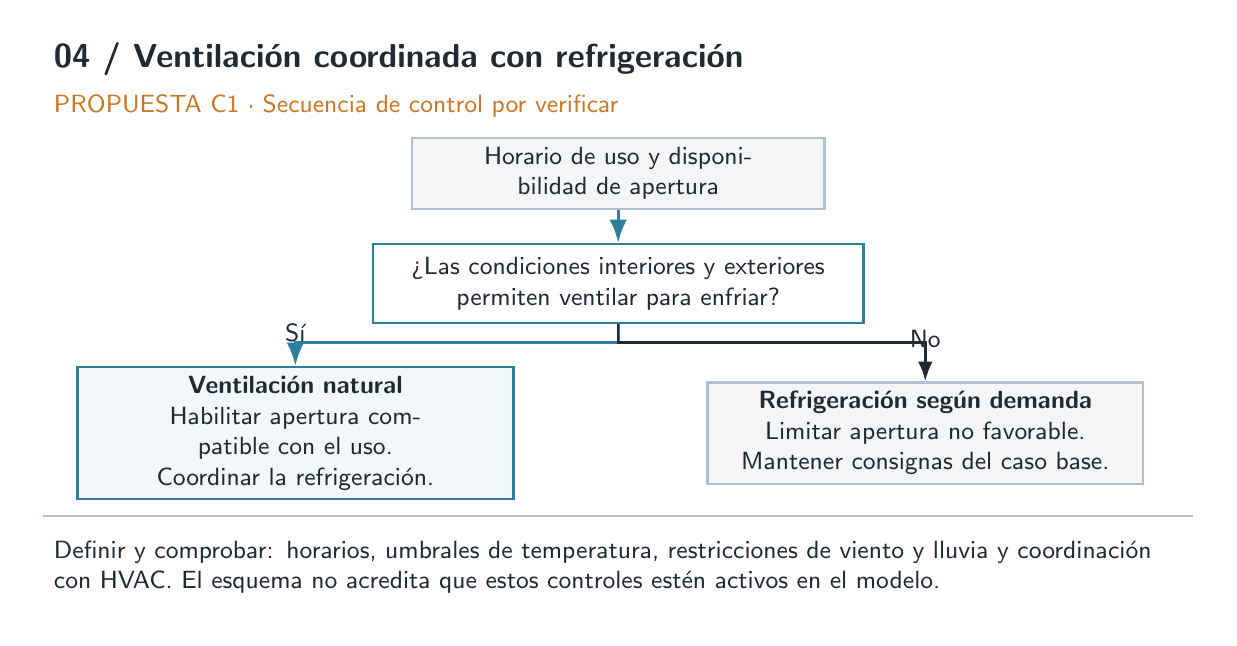
\begin{tikzpicture}[x=1cm,y=1cm,>=Latex,line width=.9pt,every node/.style={font=\sffamily\small,text=ink},note/.style={align=left,text width=4.1cm,anchor=west},flow/.style={->,blue,line width=1.2pt}]
\path[use as bounding box] (0,0) rectangle (15,7.5);

\node[anchor=west,font=\sffamily\bfseries\large] at (.2,7.1) {04 / Ventilación coordinada con refrigeración};
\node[anchor=west,text=orange] at (.2,6.5) {PROPUESTA C1 · Secuencia de control por verificar};
\node[draw=light,fill=soft,align=center,text width=5cm,minimum height=.7cm] (a) at (7.5,5.65) {Horario de uso y disponibilidad de apertura};
\node[draw=blue,align=center,text width=6cm,minimum height=1cm] (b) at (7.5,4.25) {¿Las condiciones interiores y exteriores\\permiten ventilar para enfriar?};
\node[draw=blue,fill=blue!6,align=center,text width=5.3cm,minimum height=1.1cm] (c) at (3.4,2.35) {\textbf{Ventilación natural}\\Habilitar apertura compatible con el uso.\\Coordinar la refrigeración.};
\node[draw=light,fill=soft,align=center,text width=5.3cm,minimum height=1.1cm] (d) at (11.4,2.35) {\textbf{Refrigeración según demanda}\\Limitar apertura no favorable.\\Mantener consignas del caso base.};
\draw[flow] (a)--(b);
\draw[flow] (b.south)--(7.5,3.5)-|node[above,pos=.7] {Sí} (c.north);
\draw[->,ink] (b.south)--(7.5,3.5)-|node[above,pos=.7] {No} (d.north);
\draw[light] (.2,1.3)--(14.8,1.3);
\node[anchor=west,text width=14cm,align=left] at (.2,.65) {Definir y comprobar: horarios, umbrales de temperatura, restricciones de viento y lluvia y coordinación con HVAC. El esquema no acredita que estos controles estén activos en el modelo.};

\end{tikzpicture}
\end{document}
